\documentclass[11pt,a4paper]{article}
\usepackage[margin=1in]{geometry}
\usepackage{tikz}
\usepackage{pgf-umlcd}
\usepackage{fontspec}
\usepackage{xcolor}
\usepackage{amsfonts}
\usepackage{amsmath}

% Configure emoji font for XeLaTeX (vector-based for better compatibility)
\newfontfamily\emojifont{Segoe UI Emoji}[
    Scale=1.0
]

% Create convenient emoji command
\newcommand{\emoji}[1]{{\emojifont #1}}

\usetikzlibrary{shapes,arrows,positioning,fit,backgrounds,decorations.pathmorphing,calc,shadows,matrix}

\title{PeiDocker Terminal GUI - Application Overview Design}
\author{Claude Code}
\date{\today}

\definecolor{primaryblue}{RGB}{51,122,183}
\definecolor{successgreen}{RGB}{92,184,92}
\definecolor{warningorange}{RGB}{240,173,78}
\definecolor{dangered}{RGB}{217,83,79}
\definecolor{lightgray}{RGB}{248,248,248}
\definecolor{darkgray}{RGB}{85,85,85}

\tikzset{
    % Define standard node styles
    mainbox/.style={
        rectangle, draw=primaryblue, thick, fill=lightgray,
        text width=3cm, text centered, minimum height=1.2cm,
        rounded corners=3pt, drop shadow
    },
    processbox/.style={
        rectangle, draw=successgreen, thick, fill=white,
        text width=2.5cm, text centered, minimum height=1cm,
        rounded corners=3pt
    },
    decisionbox/.style={
        diamond, draw=warningorange, thick, fill=white,
        text width=2cm, text centered, minimum height=1cm,
        aspect=2
    },
    terminalbox/.style={
        ellipse, draw=dangered, thick, fill=white,
        text width=2cm, text centered, minimum height=0.8cm
    },
    arrow/.style={
        ->, >=stealth, thick, color=darkgray
    },
    annotation/.style={
        rectangle, draw=none, fill=none,
        text width=2.5cm, font=\footnotesize,
        text=darkgray
    }
}

\begin{document}

\maketitle

\section{Application Architecture Overview}

This document provides comprehensive visual designs for the PeiDocker Terminal GUI using the Textual framework. The GUI provides two interaction modes: Simple (wizard-based) and Advanced (form-based) for creating Docker container configurations.

\subsection{High-Level Application Flow}

\begin{figure}[htbp]
\centering
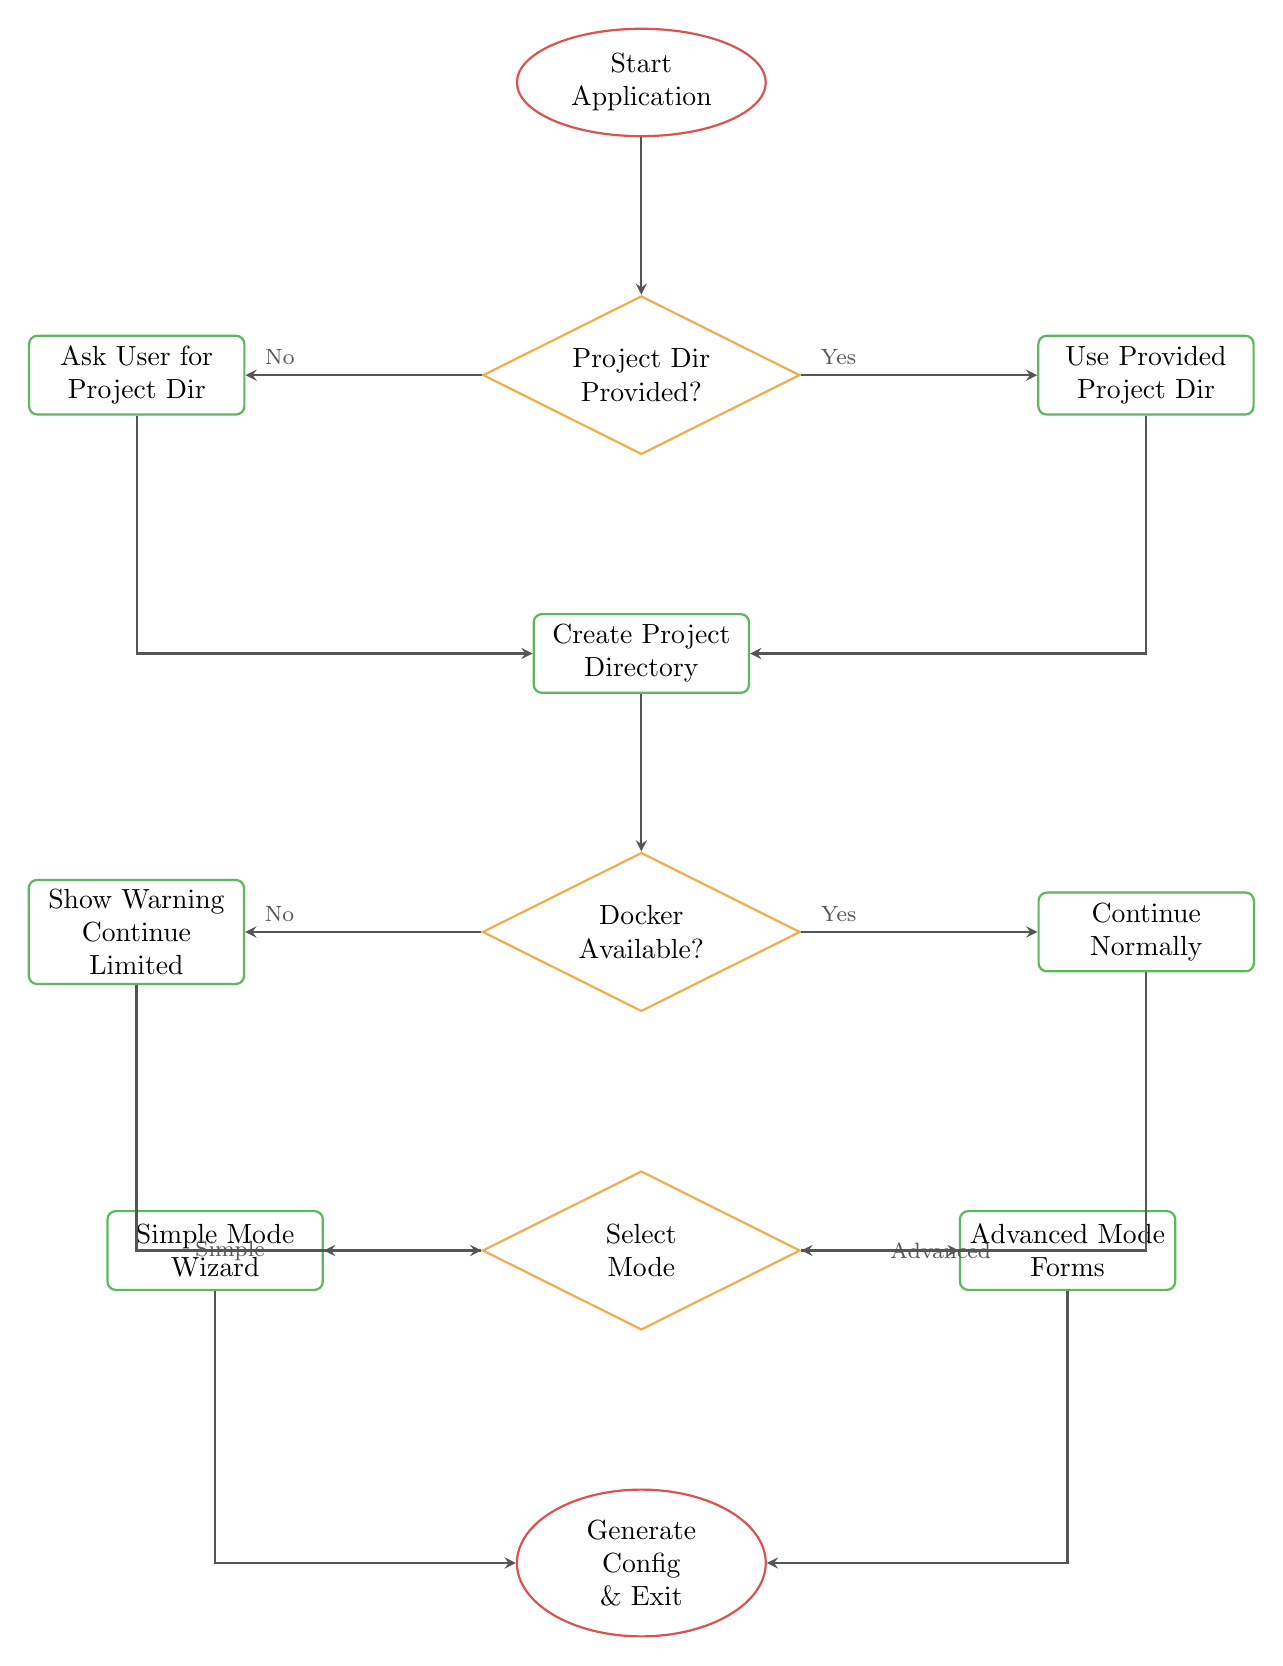
\begin{tikzpicture}[node distance=2cm and 3cm]

% Main application flow
\node[terminalbox] (start) {Start\\Application};
\node[decisionbox, below=of start] (project_dir) {Project Dir\\Provided?};
\node[processbox, right=of project_dir] (use_provided) {Use Provided\\Project Dir};
\node[processbox, left=of project_dir] (ask_project) {Ask User for\\Project Dir};
\node[processbox, below=2cm of project_dir] (create_project) {Create Project\\Directory};
\node[decisionbox, below=of create_project] (docker_check) {Docker\\Available?};
\node[processbox, right=of docker_check] (docker_ok) {Continue\\Normally};
\node[processbox, left=of docker_check] (docker_warn) {Show Warning\\Continue Limited};
\node[decisionbox, below=2cm of docker_check] (mode_select) {Select\\Mode};
\node[processbox, left=2cm of mode_select] (simple_mode) {Simple Mode\\Wizard};
\node[processbox, right=2cm of mode_select] (advanced_mode) {Advanced Mode\\Forms};
\node[terminalbox, below=2cm of mode_select] (end) {Generate\\Config \& Exit};

% Arrows
\draw[arrow] (start) -- (project_dir);
\draw[arrow] (project_dir) -- node[annotation, above] {Yes} (use_provided);
\draw[arrow] (project_dir) -- node[annotation, above] {No} (ask_project);
\draw[arrow] (use_provided) |- (create_project);
\draw[arrow] (ask_project) |- (create_project);
\draw[arrow] (create_project) -- (docker_check);
\draw[arrow] (docker_check) -- node[annotation, above] {Yes} (docker_ok);
\draw[arrow] (docker_check) -- node[annotation, above] {No} (docker_warn);
\draw[arrow] (docker_ok) |- (mode_select);
\draw[arrow] (docker_warn) |- (mode_select);
\draw[arrow] (mode_select) -- node[annotation, left] {Simple} (simple_mode);
\draw[arrow] (mode_select) -- node[annotation, right] {Advanced} (advanced_mode);
\draw[arrow] (simple_mode) |- (end);
\draw[arrow] (advanced_mode) |- (end);

\end{tikzpicture}
\caption{Main Application Flow}
\end{figure}

\subsection{Application Components Architecture}

\begin{figure}[htbp]
\centering
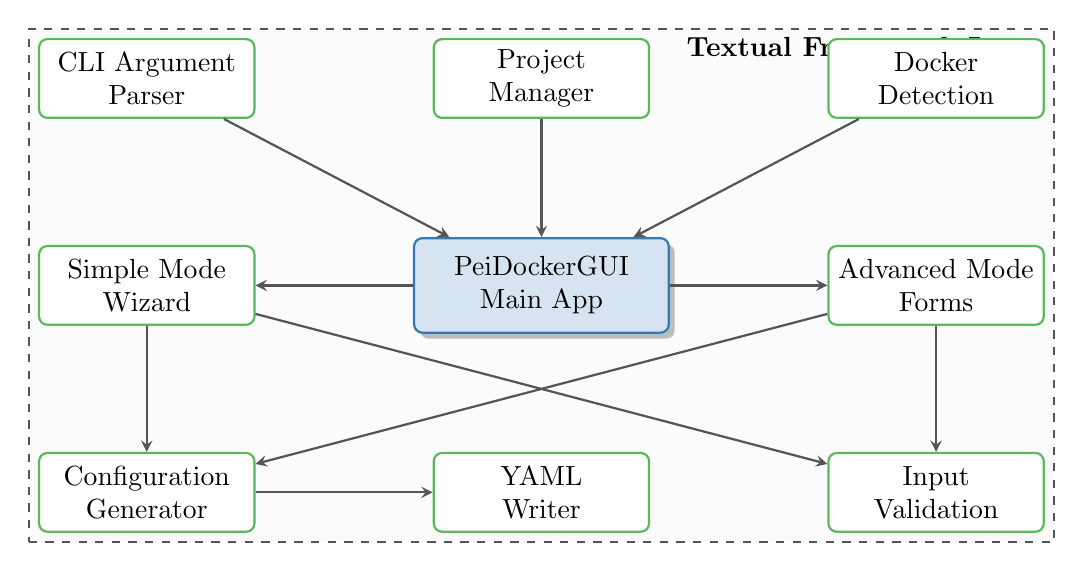
\begin{tikzpicture}[node distance=1.5cm and 2cm]

% Main application components
\node[mainbox, fill=primaryblue!20] (app) {PeiDockerGUI\\Main App};

% CLI components
\node[processbox, above left=of app] (cli_parser) {CLI Argument\\Parser};
\node[processbox, above=of app] (project_mgr) {Project\\Manager};
\node[processbox, above right=of app] (docker_detect) {Docker\\Detection};

% Mode components
\node[processbox, left=2cm of app] (simple_wizard) {Simple Mode\\Wizard};
\node[processbox, right=2cm of app] (advanced_forms) {Advanced Mode\\Forms};

% Shared components
\node[processbox, below left=of app] (config_gen) {Configuration\\Generator};
\node[processbox, below=of app] (yaml_writer) {YAML\\Writer};
\node[processbox, below right=of app] (validation) {Input\\Validation};

% Textual framework layer
\begin{scope}[on background layer]
\node[fit=(cli_parser)(docker_detect)(simple_wizard)(advanced_forms)(config_gen)(validation),
      fill=lightgray!50, draw=darkgray, dashed, thick,
      label={[anchor=north east]north east:\textbf{Textual Framework Layer}}] {};
\end{scope}

% Arrows showing relationships
\draw[arrow] (cli_parser) -- (app);
\draw[arrow] (project_mgr) -- (app);
\draw[arrow] (docker_detect) -- (app);
\draw[arrow] (app) -- (simple_wizard);
\draw[arrow] (app) -- (advanced_forms);
\draw[arrow] (simple_wizard) -- (config_gen);
\draw[arrow] (advanced_forms) -- (config_gen);
\draw[arrow] (config_gen) -- (yaml_writer);
\draw[arrow] (simple_wizard) -- (validation);
\draw[arrow] (advanced_forms) -- (validation);

\end{tikzpicture}
\caption{Application Components Architecture}
\end{figure}

\subsection{File Structure Organization}

\begin{figure}[htbp]
\centering
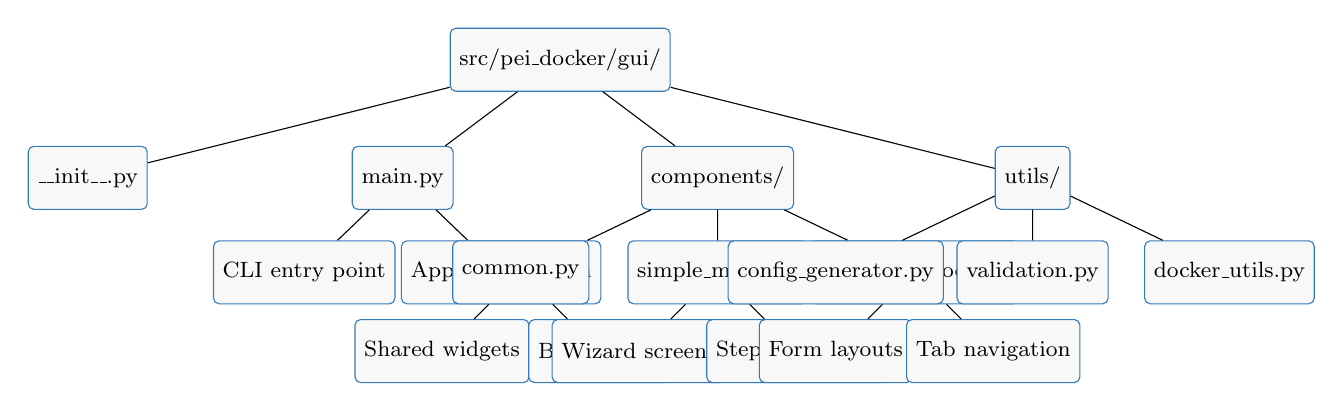
\begin{tikzpicture}[
    level 1/.style={sibling distance=4cm, level distance=1.5cm},
    level 2/.style={sibling distance=2.5cm, level distance=1.2cm},
    level 3/.style={sibling distance=2cm, level distance=1cm},
    every node/.style={
        rectangle, draw=primaryblue, fill=lightgray, 
        text centered, rounded corners=2pt,
        font=\footnotesize, minimum height=0.8cm
    }
]

\node {src/pei\_docker/gui/}
    child { node {\_\_init\_\_.py} }
    child { node {main.py}
        child { node {CLI entry point} }
        child { node {App initialization} }
    }
    child { node {components/}
        child { node {common.py}
            child { node {Shared widgets} }
            child { node {Base classes} }
        }
        child { node {simple\_mode.py}
            child { node {Wizard screens} }
            child { node {Step navigation} }
        }
        child { node {advanced\_mode.py}
            child { node {Form layouts} }
            child { node {Tab navigation} }
        }
    }
    child { node {utils/}
        child { node {config\_generator.py} }
        child { node {validation.py} }
        child { node {docker\_utils.py} }
    };

\end{tikzpicture}
\caption{Proposed File Structure}
\end{figure}

\subsection{Data Flow Architecture}

\begin{figure}[htbp]
\centering
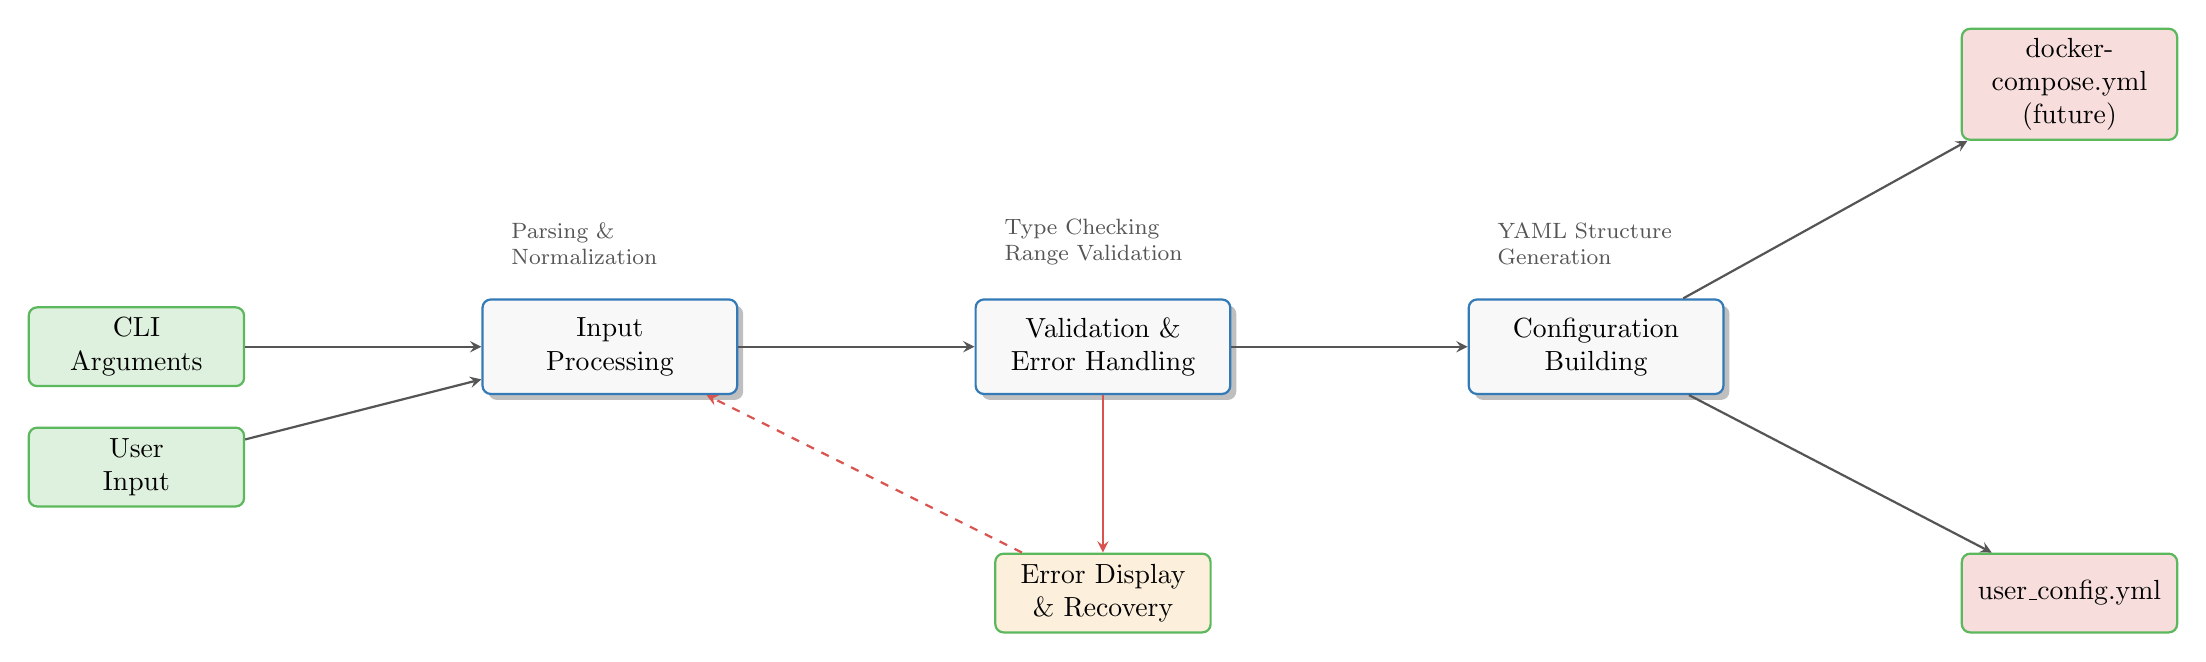
\begin{tikzpicture}[node distance=2cm and 3cm]

% Input sources
\node[processbox, fill=successgreen!20] (cli_args) {CLI\\Arguments};
\node[processbox, fill=successgreen!20, below=0.5cm of cli_args] (user_input) {User\\Input};

% Processing stages
\node[mainbox, right=of cli_args] (input_processing) {Input\\Processing};
\node[mainbox, right=of input_processing] (validation_stage) {Validation \&\\Error Handling};
\node[mainbox, right=of validation_stage] (config_build) {Configuration\\Building};

% Output destinations
\node[processbox, fill=dangered!20, below right=of config_build] (yaml_output) {user\_config.yml};
\node[processbox, fill=dangered!20, above right=of config_build] (docker_compose) {docker-compose.yml\\(future)};

% Error handling
\node[processbox, fill=warningorange!20, below=of validation_stage] (error_display) {Error Display\\\& Recovery};

% Main data flow arrows
\draw[arrow] (cli_args) -- (input_processing);
\draw[arrow] (user_input) -- (input_processing);
\draw[arrow] (input_processing) -- (validation_stage);
\draw[arrow] (validation_stage) -- (config_build);
\draw[arrow] (config_build) -- (yaml_output);
\draw[arrow] (config_build) -- (docker_compose);

% Error flow
\draw[arrow, color=dangered] (validation_stage) -- (error_display);
\draw[arrow, color=dangered, dashed] (error_display) -- (input_processing);

% Annotations
\node[annotation, above=0.3cm of input_processing] {Parsing \&\\Normalization};
\node[annotation, above=0.3cm of validation_stage] {Type Checking\\Range Validation};
\node[annotation, above=0.3cm of config_build] {YAML Structure\\Generation};

\end{tikzpicture}
\caption{Data Flow Through Application}
\end{figure}

\subsection{Mode Selection Interface}

\begin{figure}[htbp]
\centering
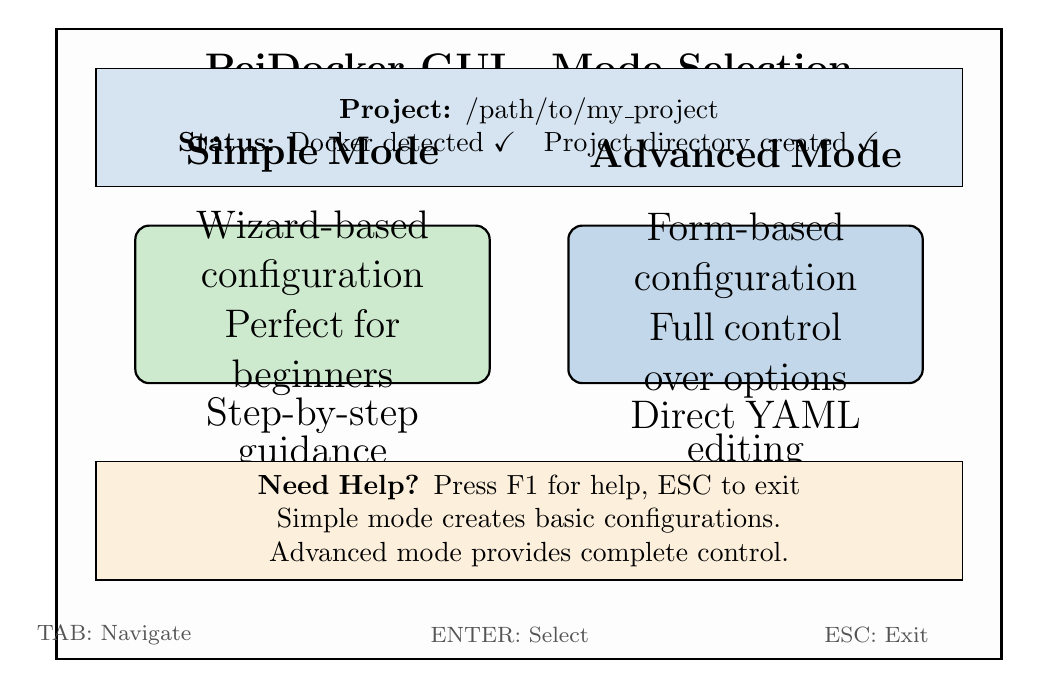
\begin{tikzpicture}

% Main window frame
\draw[thick, fill=lightgray!30] (0,0) rectangle (12,8);
\node[anchor=north] at (6,7.8) {\Large\textbf{PeiDocker GUI - Mode Selection}};

% Header section
\draw[fill=primaryblue!20] (0.5,6) rectangle (11.5,7.5);
\node[text width=10cm, text centered] at (6,6.75) {
    \textbf{Project:} /path/to/my\_project\\
    \textbf{Status:} Docker detected \checkmark \quad Project directory created \checkmark
};

% Mode selection buttons
\draw[thick, fill=successgreen!30, rounded corners=5pt] (1,3.5) rectangle (5.5,5.5);
\node[text width=4cm, text centered] at (3.25,4.5) {
    \Large\textbf{Simple Mode}\\[0.3cm]
    Wizard-based configuration\\
    Perfect for beginners\\
    Step-by-step guidance
};

\draw[thick, fill=primaryblue!30, rounded corners=5pt] (6.5,3.5) rectangle (11,5.5);
\node[text width=4cm, text centered] at (8.75,4.5) {
    \Large\textbf{Advanced Mode}\\[0.3cm]
    Form-based configuration\\
    Full control over options\\
    Direct YAML editing
};

% Help section
\draw[fill=warningorange!20] (0.5,1) rectangle (11.5,2.5);
\node[text width=10cm, text centered] at (6,1.75) {
    \textbf{Need Help?} Press F1 for help, ESC to exit\\
    Simple mode creates basic configurations. Advanced mode provides complete control.
};

% Navigation hints
\node[annotation] at (1,0.3) {TAB: Navigate};
\node[annotation] at (6,0.3) {ENTER: Select};
\node[annotation] at (11,0.3) {ESC: Exit};

\end{tikzpicture}
\caption{Mode Selection Screen Layout}
\end{figure}

\section{Technical Implementation Notes}

\subsection{Textual Framework Integration}

The GUI will be built using the Textual framework with the following key components:

\begin{itemize}
    \item \textbf{App Class}: Main application controller inheriting from \texttt{textual.app.App}
    \item \textbf{Screen Classes}: Separate screens for different phases (startup, mode selection, configuration)
    \item \textbf{Widget Classes}: Custom widgets for specialized input types (SSH keys, port mappings, etc.)
    \item \textbf{Reactive Variables}: For real-time validation and state management
    \item \textbf{CSS Styling}: For consistent visual appearance across all components
\end{itemize}

\subsection{Error Handling Strategy}

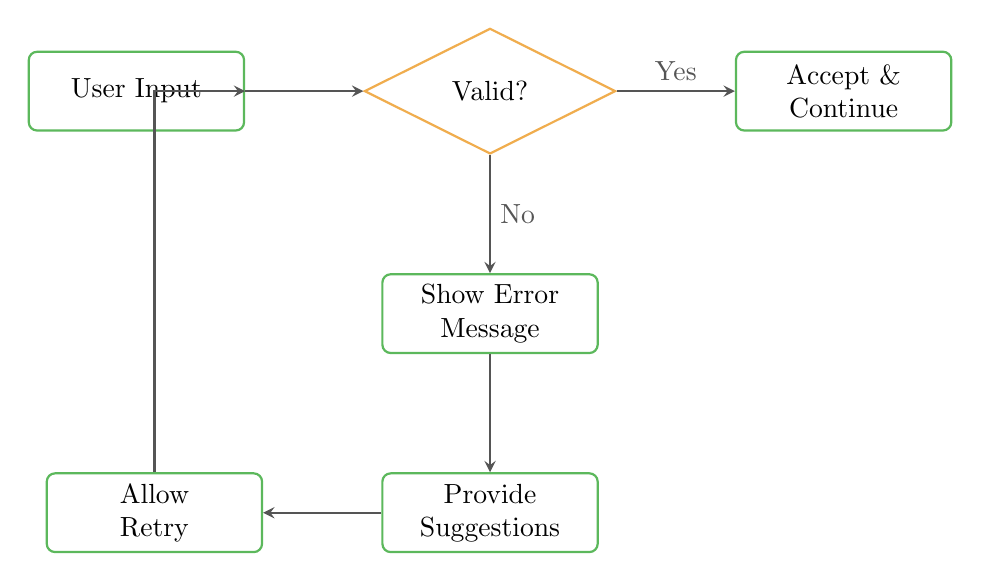
\begin{tikzpicture}[node distance=1.5cm]

\node[processbox] (input) {User Input};
\node[decisionbox, right=of input] (validate) {Valid?};
\node[processbox, right=of validate] (accept) {Accept \&\\Continue};
\node[processbox, below=of validate] (error_msg) {Show Error\\Message};
\node[processbox, below=of error_msg] (suggest) {Provide\\Suggestions};
\node[processbox, left=of suggest] (retry) {Allow\\Retry};

\draw[arrow] (input) -- (validate);
\draw[arrow] (validate) -- node[above] {Yes} (accept);
\draw[arrow] (validate) -- node[right] {No} (error_msg);
\draw[arrow] (error_msg) -- (suggest);
\draw[arrow] (suggest) -- (retry);
\draw[arrow] (retry) |- (input);

\end{tikzpicture}

\subsection{Configuration Generation Pipeline}

The application follows a structured pipeline for converting user input into the final YAML configuration:

\begin{enumerate}
    \item \textbf{Input Collection}: Gather all user inputs through GUI forms/wizards
    \item \textbf{Validation}: Check data types, ranges, and relationships
    \item \textbf{Transformation}: Convert GUI data structures to config objects
    \item \textbf{Template Application}: Apply user data to configuration templates
    \item \textbf{YAML Generation}: Serialize final configuration to YAML format
    \item \textbf{File Writing}: Save configuration to project directory
\end{enumerate}

\end{document}